\documentclass[11pt]{article} % DO NOT CHANGE THIS

% DO NOT CHANGE ANYTHING IN THE FOLLOWING BLOCK
%%%%%%%%%%%%%%%%%%%%%%%% BLOCK START %%%%%%%%%%%%%%%%%%%%%%%%

\usepackage{fullpage}
\usepackage{amsmath,amssymb,amsthm}
\usepackage[roman,full]{complexity}
\usepackage{tabularx,booktabs}
\usepackage{graphicx}
\graphicspath{{../figures/}}
\usepackage{subcaption}
\usepackage[
    style=apa,
    backend=biber,
    doi=true,
    url=true
]{biblatex}
\usepackage{hyperref}

\addbibresource{references.bib}

\hypersetup{
    colorlinks=true,
    citecolor=blue,
    linkcolor=blue,
    urlcolor=blue
}


%%%%%%%%%%%%%%%%%%%%%%%%% BLOCK END %%%%%%%%%%%%%%%%%%%%%%%%%

% You can add your own command/packages/environments below

%%%Definition
\newcommand{\LANGDEF}[3]{
\begin{center}
{\small 
\begin{tabularx}{0.98\columnwidth}{ll}
\toprule
\multicolumn{2}{c}{\textsc{#1}} \\
\midrule
{\bf Given:}   & \parbox[t]{0.75\columnwidth}{#2\vspace*{1mm}}  \\
{\bf Question:}& \parbox[t]{0.75\columnwidth}{#3\vspace*{.5mm}} \\ 
\bottomrule
\end{tabularx}
}
\end{center}
}

\newcommand{\OPTDEF}[4]{
\begin{center}
{\small 
\begin{tabularx}{0.98\columnwidth}{ll}
\toprule
\multicolumn{2}{c}{\textsc{#1}} \\
\midrule
{\bf Given:}   & \parbox[t]{0.75\columnwidth}{#2\vspace*{1mm}}  \\
{\bf Solution:}& \parbox[t]{0.75\columnwidth}{#3\vspace*{.5mm}} \\ 
{\bf Measure:}& \parbox[t]{0.75\columnwidth}{#4\vspace*{.5mm}} \\ 
\bottomrule
\end{tabularx}
}
\end{center}
}

\newcommand{\km}{\text{km}}


%%% MATH THINGS
\newtheorem{theorem}{Theorem}[section]
\newtheorem{claim}[theorem]{Claim}
\newtheorem{lemma}[theorem]{Lemma}
\newtheorem{proposition}[theorem]{Proposition}
\newtheorem{remark}[theorem]{Remark}
\newtheorem{observation}[theorem]{Observation}
\newtheorem{construction}[theorem]{Construction}
\newtheorem{corollary}[theorem]{Corollary}

% \theoremstyle{definition}
\newtheorem{definition}[theorem]{Definition}


\title{Application of NPP-VIIRS Nighttime Light Imagery for GDP Spatialization and Economic Differences in Vietnam\\
\Large DA~401 Early Results}
\author{Kien Le T.}
\date{\today}


\begin{document}

\maketitle

\section{Introduction}

\emph{Gross domestic product} (GDP) is a fundamental economic indicator within a country or region. More detailed GDP estimates can provide researchers and policymakers with a clearer understanding of regional economic disparities and development patterns. However, conventional socioeconomic statistics used to measure GDP often suffer from inconsistent statistical scales and limited spatial resolution, making it difficult to capture regional economic disparities at a fine spatial scale. Therefore, many studies have proposed various methods for constructing maps and data on regional GDP with respect to real world coordinates. Researchers have shown that \emph{nighttime light} (NTL) data are a useful economic indicator and have adopted and developed methods for spatializing GDP using NTL data, including both statistical and machine learning approaches. However, applications of NTL data for GDP spatialization in Vietnam remain limited, motivating this study to spatialize regional GDP in Vietnam using NTL data.

Remote sensing imagery offers clear advantages over conventional socioeconomic statistics for describing the spatial GDP distribution. Before \emph{Visible Infrared Imaging Radiometer Suite} (VIIRS) data, carried by the \emph{Suomi National Polar-Orbiting Partnership} (NPP), became available in 2013, researchers primarily relied on NTL data from the \emph{Defense Meteorological Satellite Program-Operational Linescan System} (DMSP-OLS). These studies found a strong relationship between NTL intensity and regional GDP. For example,~\textcite{elv-bau-kih:US-GDP-NTL} found a strong correlation between the area lit and GDP across 21 counties in North America using DMSP-OLS NTL data. Similar studies conducted on the data from the United States, Europe, and China have also reported strong relationships between NTL and GDP~\parencite{dol-mul-mor:EU-GDP-NTL, zha-cur-sam:CN-GDP-NTL, for:US-GDP-NTL}.

Following the introduction of NPP-VIIRS data in 2013, research increasingly shifted toward using this newer dataset~\parencite{li-xu-che:potential-VIIRS,zha-che-zho:SouthCN-GDP-NTL}. NPP-VIIRS provides higher spatial resolution (approximately 500 m) than DMSP-OLS data (1 \km), while its wider radiometric detection range reduces saturation and its onboard radiometric calibration improves data quality~\parencite{elv-bau-zhi:VIIRS-DMSP}. However, NPP-VIIRS imagery is a preliminary product affected by various sources of light, including cities, transportation corridors, gas flares, biomass burning, background noise, and reflections from bright surfaces such as snow covered mountains and playa lake beds~\parencite{elv-bau-zhi:VIIRS-DMSP}. To address these issues,~\textcite{zha-che-zho:SouthCN-GDP-NTL} proposed a method for correcting VIIRS nighttime light data. Building upon the procedure developed by~\textcite{zha-che-zho:SouthCN-GDP-NTL},~\textcite{xu-zha-jia:CN-GDP-NTL-LC} estimated regional GDP for all provinces and prefectures in China while incorporating land cover data. Their results also highlighted the effectiveness of \emph{Geographically Weighted Regression} (GWR) in capturing economic development using NTL data. The GWR model explained up to 93\% of the variation in economic development, compared with 82\% explained by the \emph{Ordinary Least Squares} (OLS) model~\parencite{xu-zha-jia:CN-GDP-NTL-LC}.~\textcite{liu-liu-zho:map-GDP-NTL-ML} used NPP-VIIRS nighttime light and land use data to develop a 1 \km gridded GDP dataset for China using machine learning methods, achieving an $R^2 = 0.78$ and providing a more detailed representation of regional economic disparities.

For Vietnam, several studies have also used NTL data to analyze and predict economic indicators. Since official GDP data for Vietnam have only been available from 2010 onward,~\textcite{sul-ngu-men:VN-GDP-NTL-ML} estimated Vietnam's subnational GDP from 1992 to 2010 using NTL data, demonstrating that remote sensing data can serve as a reliable predictor of Vietnam subnational GDP. In addition to that,~\textcite{zha:VN-GDP-disparities} demonstrated that NTL data can effectively capture spatial economic disparities patterns in Vietnam, particularly by identifying clusters of economically developed and underdeveloped regions. These findings suggest that the relationship between NTL data and economic activity observed in other regions also holds in Vietnam, providing a strong basis for applying NTL methods for GDP spatialization. However, to the best of my knowledge, no existing study has applied NTL data to spatialize Vietnam's GDP at the regional level, although similar applications have been conducted at the global level~\parencite{wan-sut-qi:Global-GDP-VIIRS}.

Therefore, this study aims to address this gap by adapting and extending the methods used in previous research to spatialize regional GDP in Vietnam using NPP-VIIRS NTL data. In addition, this research will develop an automated and reproducible analytical workflow that takes NPP-VIIRS imagery and regional GDP data as inputs and produces spatial GDP estimates.

\section{Materials and Methods}

\subsection{Study Area}

In this study, I analyze the Gross Regional Domestic Product (GRDP) of provinces and centrally governed cities in Vietnam, which span latitudes from $8^\circ 10' \mathrm{N}$ to $23^\circ 24' \mathrm{N}$ and longitudes from $102^\circ 09' \mathrm{E}$ to $109^\circ 30' \mathrm{E}$. Vietnam has a total land area of approximately 331,212~$\km^2$, of which mountains, plateaus, and hills account for approximately three-quarters. According to the National Statistics Office of Vietnam (NSO), Vietnam's GDP reached  12,847.6 billion VND (approximately USD 514 billion) in 2025, reflecting a growth rate of 5.67\%\footnote{This number is calculated by using Vietnam's GDP from 2025 and 2017, where Vietnam's GDP is according to NSO.
} during the 2020--2025 period. Economic development across Vietnam's regions is highly uneven and the country's rapid economic growth has created significant regional disparities.~\textcite{zha:VN-GDP-disparities} documented substantial spatial heterogeneity in Vietnam's economic development: major urban centers such as Hanoi, Ho Chi Minh City, and Hai Phong experienced rapid growth, whereas regions such as the Northwest and the Mekong Delta developed at a comparatively slower pace.

An important consideration for this study is the recent change in Vietnam's provincial level administrative boundaries. On June 12, 2025, the Vietnamese National Assembly passed Resolution No.~202/2025/QH15, reducing the number of provincial level administrative units from 63 to 34, consisting of 28 provinces and 6 centrally governed municipalities. Therefore, this analysis will be adjusted according to the new boundaries.

\subsection{Data}

This study utilizes data from three sources. First, the primary indicator, \emph{Gross Regional Domestic Product} (GRDP), is obtained from the Statistical Yearbook of Viet Nam 2025, covering the period from 2020 to 2025. The NSO also provides data on national GDP, GRDP by capita, population, and population density across regions of Vietnam. Second, NTL data are obtained from the \emph{Earth Observation Group} (EOG) and are derived from VIIRS observations collected aboard the Suomi NPP satellite, part of the \emph{Joint Polar Satellite System} (JPSS), covering the period from 2012 to 2025. Third, administrative boundary shapefiles are obtained through the Humanitarian Data Exchange portal, provided by the \emph{United Nations Office for the Coordination of Humanitarian Affairs} (OCHA). According to the boundary dataset documentation, the boundary alignments incorporate the latest updates from official Vietnamese government decrees. For the commune-level boundary shapefile, I collect from \href{https://gis.vn/}{gis.vn}, a Vietnamese geospatial platform and community tool.

\subsubsection{National Statistics Office of Vietnam}

GRDP data for the 34 provinces and centrally governed municipalities in Vietnam covering the period from 2020 to 2025 were obtained from the 2025 Statistical Yearbook. The yearbook is an annual publication issued by the National Statistics Office of Vietnam (NSO) and is available through the official NSO website. The GRDP figures reported in the 2025 edition are the first to be calculated according to Vietnam's new provincial administrative classification. These figures are reported at constant prices, with 2010 as the base year, and therefore adjusted for inflation. In previous editions, GDP was reported according to the former provincial administrative classification. The GDP figures are expressed in constant local currency values.

For population data, the annual national statistical yearbooks provide population and population density estimates at the provincial level. In addition, the statistical yearbooks published by individual provinces provide population data at a finer geographic level, including the commune level. However, GRDP data are not available at the provincial and commune level. Therefore, population data can be incorporated into the analysis at both the provincial and commune levels.

\subsubsection{Nighttime Light data preprocessing}

The data is obtained in GeoTIFF format. Here, I will use the Annual VNL V2 dataset for 2020--2025 because it has already undergone processing to reduce the effects of outliers and temporary light sources~\parencite{elv-zhi-gho:VIIRS-2012-2019}. The NTL data is clipped to Vietnam's administrative boundary using the administrative boundary data. Then, I extracted the radiance value of each pixel. The radiance value, measured in $\text{nW}/\text{cm}^2/\text{sr}$, represents the intensity of nighttime illumination at each location and will serve as the primary predictor in the models. The pixel level NTL data will then be spatially aggregated to the corresponding administrative units at both the provincial and commune levels. These measures will then be joined with the corresponding province GDP for model training and evaluation. The pixel level NTL will also be used for spatialization of the GDP throughout Vietnam.

\subsection{Methods}

The procedure for spatializing GDP consists of two steps. First, I will develop and evaluate predictive models at the provincial level using NTL and population data. The model predictions will then be validated against observed provincial GRDP figures to compare alternative modeling approaches and identify the model that provides the most accurate estimates of provincial GDP. Second, after selecting the optimal model based on its provincial level predictive performance, I will apply the same model specification to NTL and population data at the commune level within each province. This allows the estimated provincial GDP to be further disaggregated among individual communes based on their observed NTL and population. In this way, the provincial level model serves as the basis for generating commune level GRDP estimates, providing a much finer spatial representation of economic activity than is available in standard statistical reports.

\subsubsection{Predictive models}

In order to develop the predictive model, this study will employ several regression and machine learning algorithms to predict provincial GDP. One promising model is the Geographically Weighted Regression (GWR).~\textcite{xu-zha-jia:CN-GDP-NTL-LC} showed that the GWR model explained up to 93\% of the variation in economic development in China. Building on this approach, this study will apply GWR to Vietnam data and evaluate its ability to predict provincial GDP. To provide additional alternatives and comparisons, this study will also employ \emph{Ordinary Least Squares} as a baseline model, along with \emph{Ridge Regression} and \emph{Neural Network}. These algorithms are chosen because they are either conventional econometric methods or they can recognize complex patterns and relationships.

GWR assumes the hypothesis that the closer two observations are geographically, the more similar the influence of the explanatory variables on the dependent variable, i.e. the closer the coefficients of the explanatory parameters of the regression. The model can be written as

\begin{equation}
y_i = \beta_0(u_i,v_i) +\sum_{k}^{p}\beta_k (u_i,v_i)x_{i,k} + \varepsilon_i
\end{equation}

where the coefficients at the point of geographic coordinates are
\begin{equation}
\hat\beta (u_i,v_i) = (\mathbf{X}^\top \mathbf{W}_{(\mathbf{u}_i,\mathbf{v}_i)} \mathbf{X})^{-1} \mathbf{X}^\top \mathbf{W}_{(\mathbf{u}_i,\mathbf{v}_i)} \mathbf{Y} 
\end{equation}

The importance of remote observations is weighted according to the matrix W, determined by the choice of the kernel function with the fixed bandwidth. The GWR models will be implemented using the \texttt{GWmodel} package in R~\parencite{gol-lu-char:GWmodel}.

In order to evaluate the predictive power of these models, I will use the temporal holdout approach. Data from 2020 to 2024 will be used as the training set, while data from 2025 will be reserved as the testing set. Within the training set, k-fold cross-validation will be used for model selection and hyperparameter tuning. In each fold, the model will use NTL, area, and population as predictors to estimate provincial GDP, while the reported provincial GRDP will serve as the observed outcome. Model performance within the cross-validation procedure will be evaluated using prediction error metrics such as mean squared error (MSE). After the optimal model and hyperparameters have been identified through cross-validation, the selected model will be retrained using the complete 2020-2024 training dataset. The final model will then be applied to the previously unseen 2025 data. Its predictive performance will be evaluated using R-squared and MSE by comparing the predicted provincial GDP values with the reported 2025 GRDP values. Because the 2025 data are not used during model training, cross-validation, or hyperparameter selection, this temporal holdout approach provides an independent assessment of how well the models generalize to a new year and helps reduce the risk of overfitting.

Prior to applying these models, to account for other factors that may be associated with subnational GDP, potential control variables will include population and national GDP, as these factors may influence both economic activity and nighttime light intensity. The models will first be estimated using the control variables and then with NTL variables included to examine whether the addition of NTL information improves predictive performance. The contribution of NTL will be assessed by comparing model performance across these specifications using R-squared and MSE.

\subsubsection{GDP spatialization}

After selecting the optimal models and their corresponding parameters, the final models will be retrained using the complete available training dataset. These models will then be used to estimate GDP at the commune level. This disaggregation treats each province as the higher-level geographic unit and its constituent communes as the lower-level units. Commune-level NTL, population, and other model inputs will be used to estimate the relative economic activity of each commune within its province.

An important assumption is that the disaggregation from national level down to provincial level is similar to the disaggregation from provincial level to commune level. To ensure consistency between geographic levels, the commune-level estimates will be subject to an aggregation constraint such that the sum of the estimated GDP across all communes within a province equals the corresponding provincial GDP. This constraint ensures that the resulting GDP estimates are spatially disaggregated estimates of provincial GDP rather than unconstrained independent predictions, while maintaining consistency with the higher-level provincial estimates.

With respect to the GWR models, bandwidth selection must be adjusted to reflect the different spatial scales of the provincial and commune. The geographic distances between communes are much smaller than between provinces, resulting in different spatial relationships and therefore different optimal bandwidths. Also need to note that there is a substantial regional disparities across Vietnam, which can strongly influence the optimal bandwidth at the provincial level. 

\subsubsection{Outliers}

A potential source of bias in the relationship between NTL and GDP is the presence of dragon fruit production, since lighting is used extensively to support dragon fruit cultivation. Lam Dong is a major dragon fruit production region in Vietnam, making this province a potential outlier in the model. Therefore, Lam Dong will be carefully examined during model development. I will conduct sensitivity analyses with and without Lam Dong in the training data to assess its influence on model coefficients and predictive performance. If its influence is substantial, the final model specification will account for this outlier rather than allowing its unusually high NTL values to disproportionately affect GDP estimates.

\section{Results}

\subsection{Preliminaries}

For convenience, we refer to the national, provincial, and commune levels as Level 0, Level 1, and Level 2, respectively. For each model, define the following notation:
\begin{itemize}
    \item \(y \in \mathbb{R}^n\): the vector of observed outcomes, representing GRDP per capita.
    \item \(x_i \in \mathbb{R}^3\): the vector of standardized explanatory variables for observation \(i\), comprising \texttt{mean\_radiance}, \texttt{population}, and \texttt{pixel\_count}.
    \item \(P_i\): the population associated with observation \(i\) at the corresponding administrative level.
    \item \(a \in \mathbb{R}\): the specified aggregate GDP or GRDP at the corresponding administrative level.
\end{itemize}

\subsection{Linear Regression Model}
\label{sec:linear_regression_model}

The linear model is formulated as the following constrained optimization problem:
\[
\begin{aligned}
\min_{\alpha,\beta}\quad
& \|y-\hat{y}\|_2^2\\
\text{subject to}\quad
& \sum_{i:\,\mathrm{year}_i=t} P_i\hat{y}_i=a_t,
\quad t\in\{2020,\ldots,2025\},\\
& \hat{y}_i=\alpha_{\mathrm{year}_i}+x_i^\top\beta.
\end{aligned}
\]
The objective function is identical to that of ordinary least squares (OLS), minimizing the sum of squared differences between observed and predicted GRDP per capita. However, I introduce additional equality constraints to ensure that the predictions are consistent with the reported aggregate economic output at the national level for each year. That is, the sum of products of population and predicted GRDP per capita must equal the corresponding reported aggregate GDP, as enforced by the first constraint.

For the level 2 predictions, I apply the following adjustment to the model predictions to ensure consistency with the reported provincial GRDP per capita:
\[
\tilde{y}_{ij}=\hat{y}_{ij}+\delta_j,
\]
where
\[
\delta_j=
\frac{
g_jN_j-\displaystyle\sum_{i\in j}P_{ij}\hat{y}_{ij}
}{
\displaystyle\sum_{i\in j}P_{ij}
}.
\]
Here, \(\delta_j\) is the common adjustment term for every level 2 prediction within province \(j\), \(g_j\) denotes the reported GRDP per capita of province \(j\) in 2025, \(N_j\) is the province's reported total population, and \(P_{ij}\) is the population of commune \(i\) within province \(j\). This adjustment distributes the difference between the reported provincial GRDP and the aggregate implied by the original commune-level predictions proportionally to population, while preserving the relative differences among the original predictions.

Consequently, the adjusted predictions satisfy the following aggregation constraint for each province \(j\):
\[
\sum_{i\in j}P_{ij}\tilde{y}_{ij}=g_jN_j.
\]

\subsubsection{Statistical analysis}
A natural way to evaluate the impact of the constraints is to compare the RMSE and \(R^2\) of the constrained and unconstrained linear models, as summarized in Table \ref{tab:model_comparison}.

\begin{table}[htbp]
    \centering
    \caption{Model Performance Comparison}
    \label{tab:model_comparison}
    \begin{tabular}{lrr}
        \hline
        Model & $R^2$ & RMSE \\
        \hline
        Constrained Regression & 0.4712128 & 29.03304 \\
        Ordinary Least Squares & 0.4730061 & 28.98377 \\
        \hline
    \end{tabular}
\end{table}

We can see that imposing the aggregation constraints has a negligible impact on predictive performance. Compared with OLS, the constrained regression increases the RMSE by only \(0.17\%\), while \(R^2\) decreases slightly from $0.4730$ to $0.4712$. Thus, the different between the constrained and the unconstrained model are minimal

\subsection{Predictions at a finer spatial scale}

\begin{figure}[htbp]
    \centering
    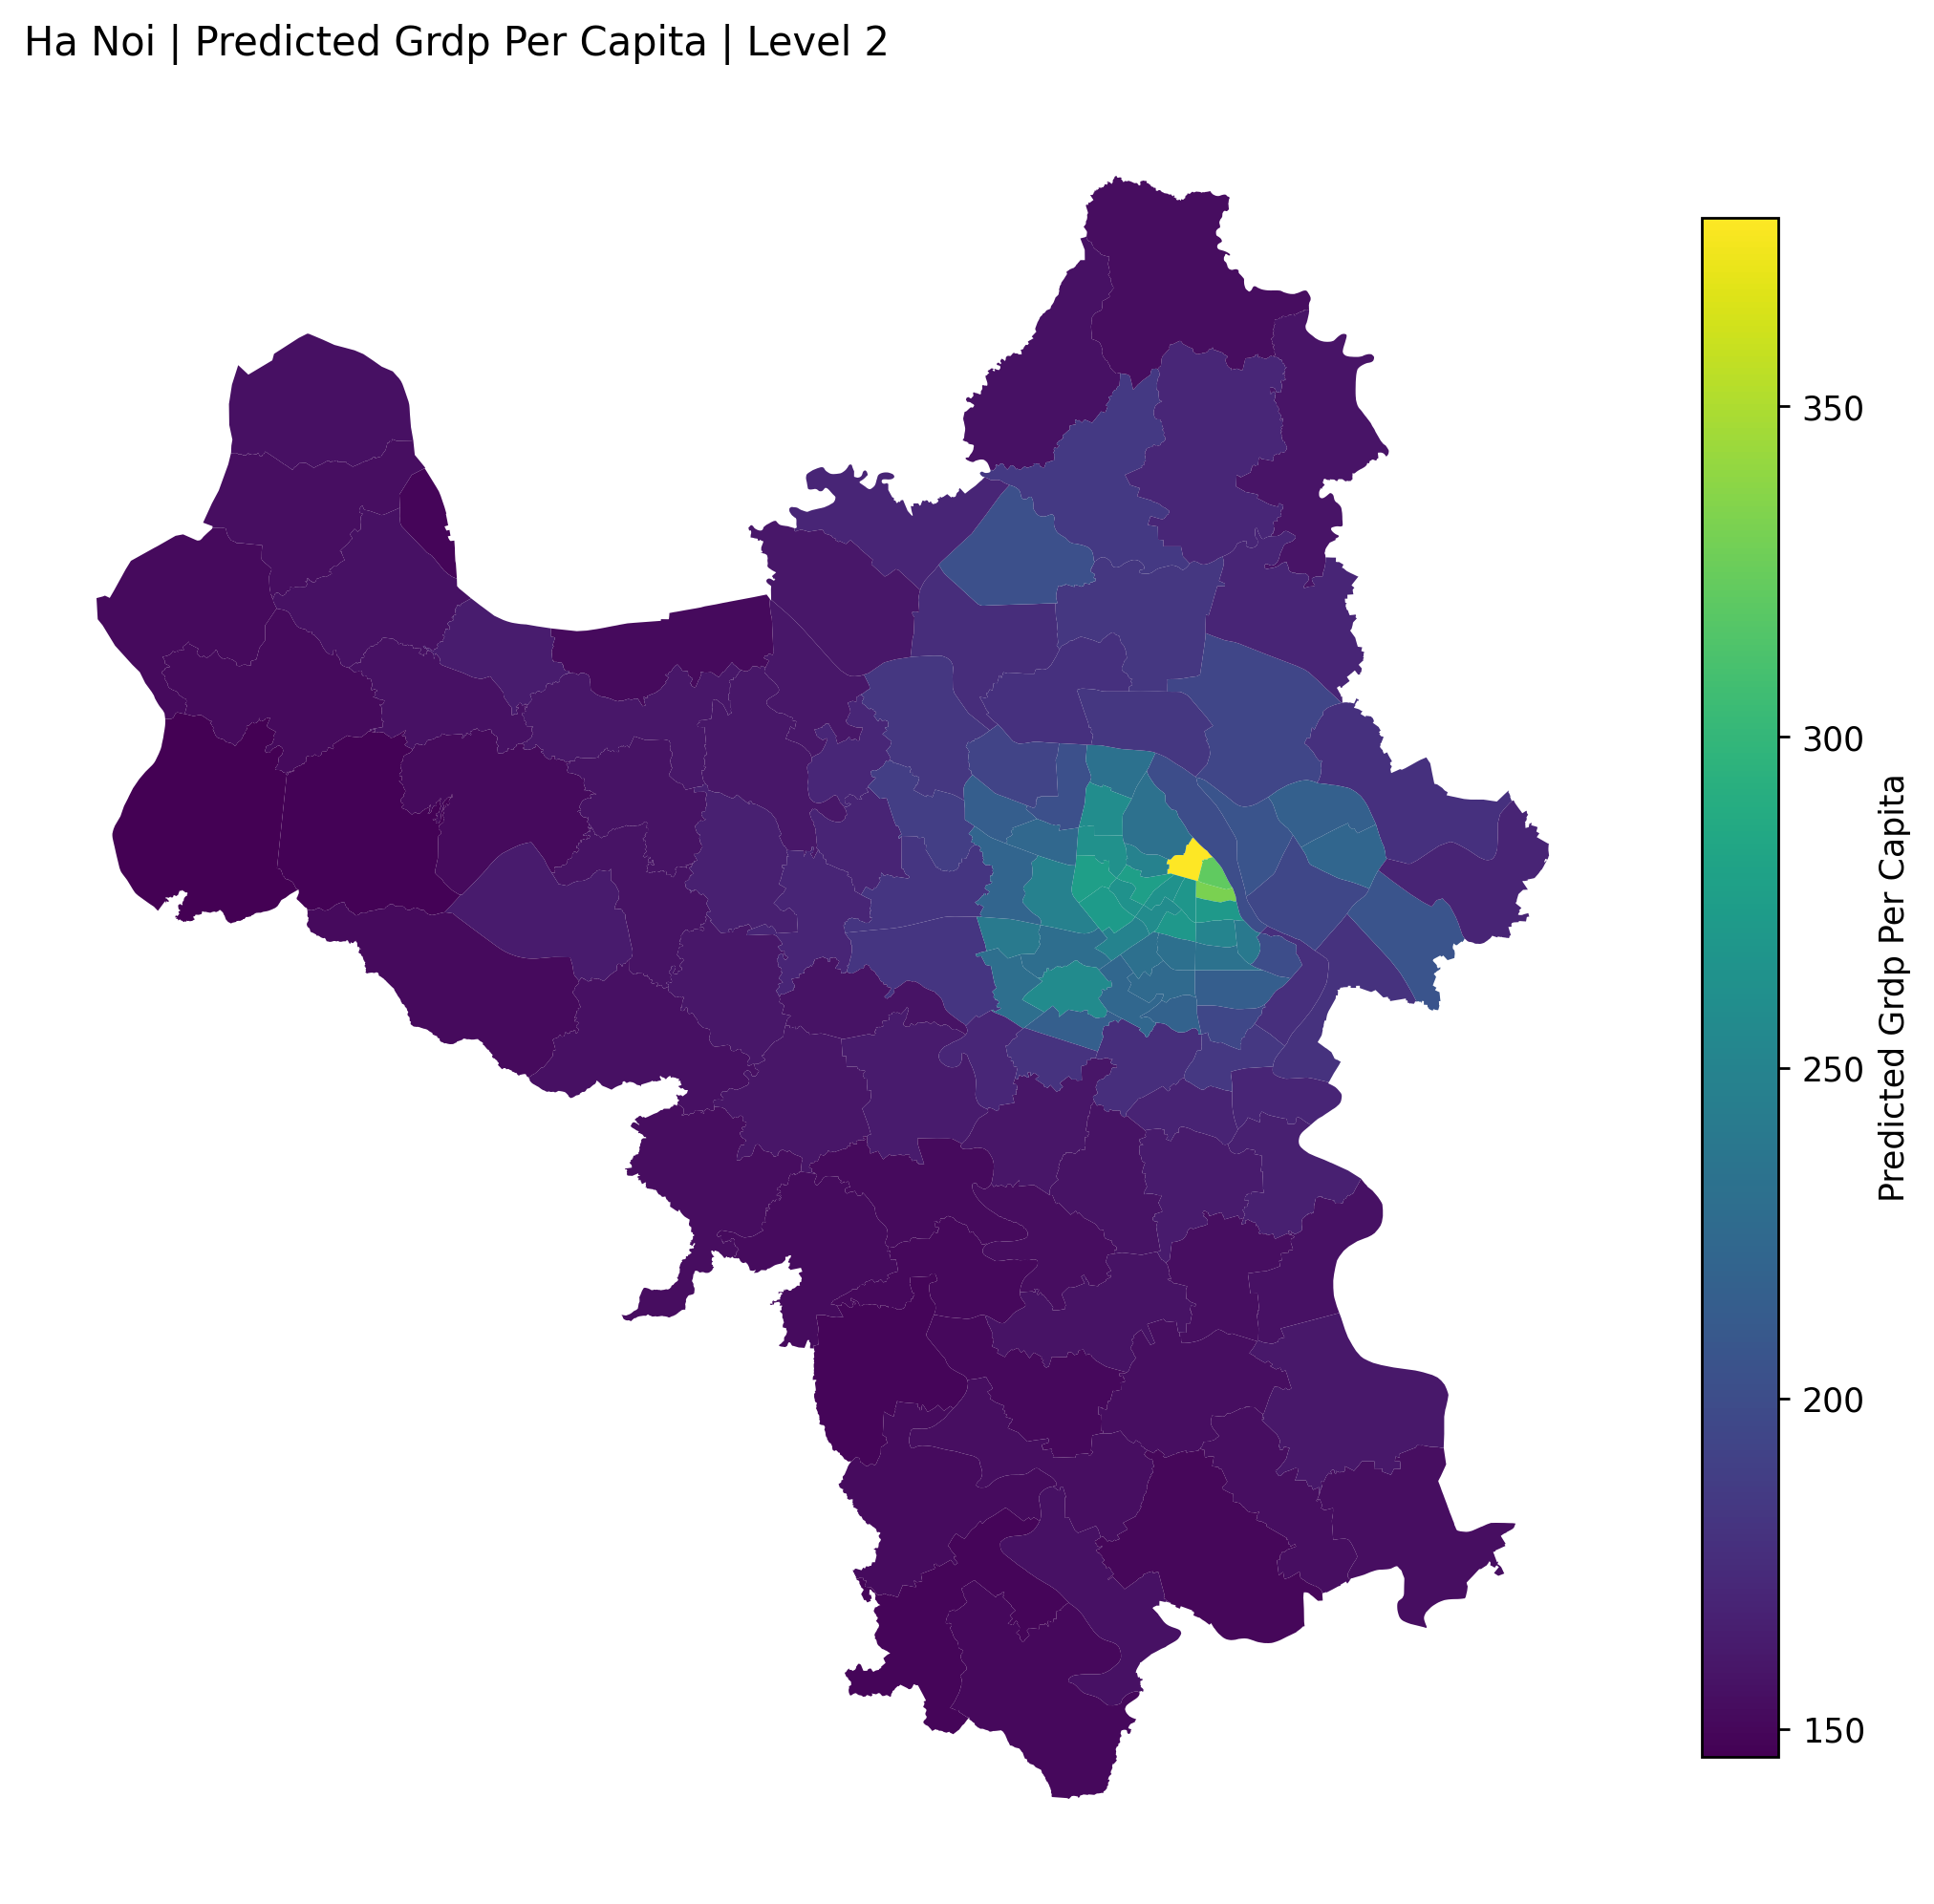
\includegraphics[width=0.5\linewidth]{ha_noi_level2_predicted_grdp_per_capita.png}
    \caption{Predicted GRDP per capita at the commune level in Ha Noi}
    \label{fig:ha_noi_level2_predicted_grdp_per_capita}
\end{figure}

Figure \ref{fig:ha_noi_level2_predicted_grdp_per_capita} shows the estimated GRDP per capita at level 2 in Ha Noi. The spatialization results reveal a plausible geographic pattern, with higher predicted GRDP per capita concentrated in the city center. This pattern is consistent with the concentration of economic activities in urban areas.

\subsection{Ridge Regression Model}

Similar to the linear regression model, the ridge regression model can be formulated as the following constrained optimization problem:

\[
\begin{aligned}
\min_{\alpha,\beta}\quad
& \|y-\hat{y}\|_2^2+\lambda\|\beta\|_2^2\\
\text{subject to}\quad
& \sum_{i:\,\mathrm{year}_i=t}P_i\hat{y}_i=a_t,
\quad t\in\{2020,\ldots,2025\},\\
& \hat{y}_i=\alpha_{\mathrm{year}_i}+x_i^\top\beta,\\
& \lambda\geq 0.
\end{aligned}
\]

The parameter \(\lambda\) controls the strength of regularization. When \(\lambda=0\), the objective function reduces to that of the constrained linear regression model.

The adjustment procedure for Level 2 predictions is identical to that described in Section \ref{sec:linear_regression_model}.

To select the regularization parameter \(\lambda\), I evaluate model performance across a grid of values, using the temporal holdout approach. As shown in Figure \ref{fig:ridge_lambda_grid_metrics}, the best predictive performance occurs when \(\lambda = 15.85\). This suggests that penalizing the regression coefficients does improve predictive accuracy in this application, but minimally.

\begin{figure}[htbp]
    \centering
    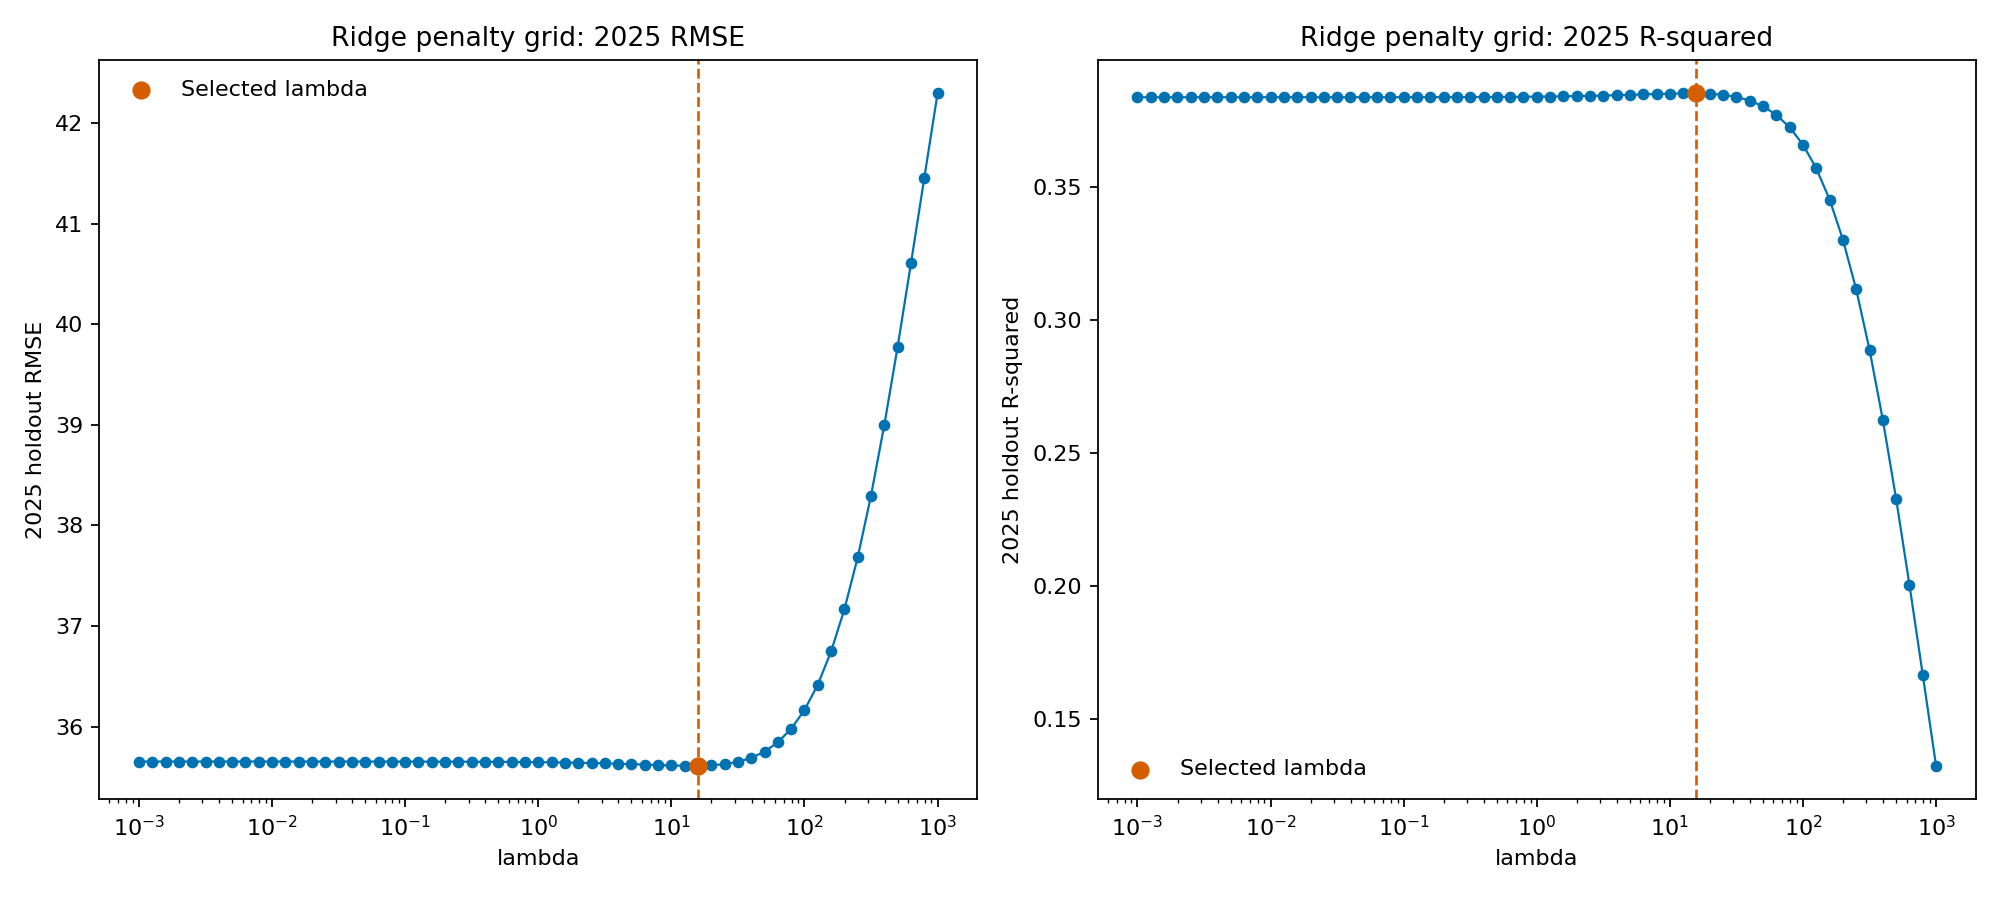
\includegraphics[width=\linewidth]{ridge_lambda_grid_metrics.png}
    \caption{RMSE and \(R^2\) across candidate values of the ridge regularization parameter \(\lambda\).}
    \label{fig:ridge_lambda_grid_metrics}
\end{figure}

\section{Outlier Problem}

Using ridge regression with a tuned $\lambda$, I estimate GRDP per capita for each commune. Figure~\ref{fig:level_1_ridge_predictions_2025} and~\ref{fig:level_2_ridge_predictions_2025}  presents the holdout predictions at two administrative levels. At Level 1, the predicted values are reasonable, with Ho Chi Minh City and Ha Noi having the highest estimated GRDP per capita. However, the Level 2 predictions reveal a potential outlier problem. Lam Dong exhibits an exceptionally high estimated GRDP per capita, with nighttime lights from dragon fruit farms potentially contributing to this result. The predicted value is disproportionately high, even compared with those of the country's two largest cities.

\begin{figure}
    \centering
    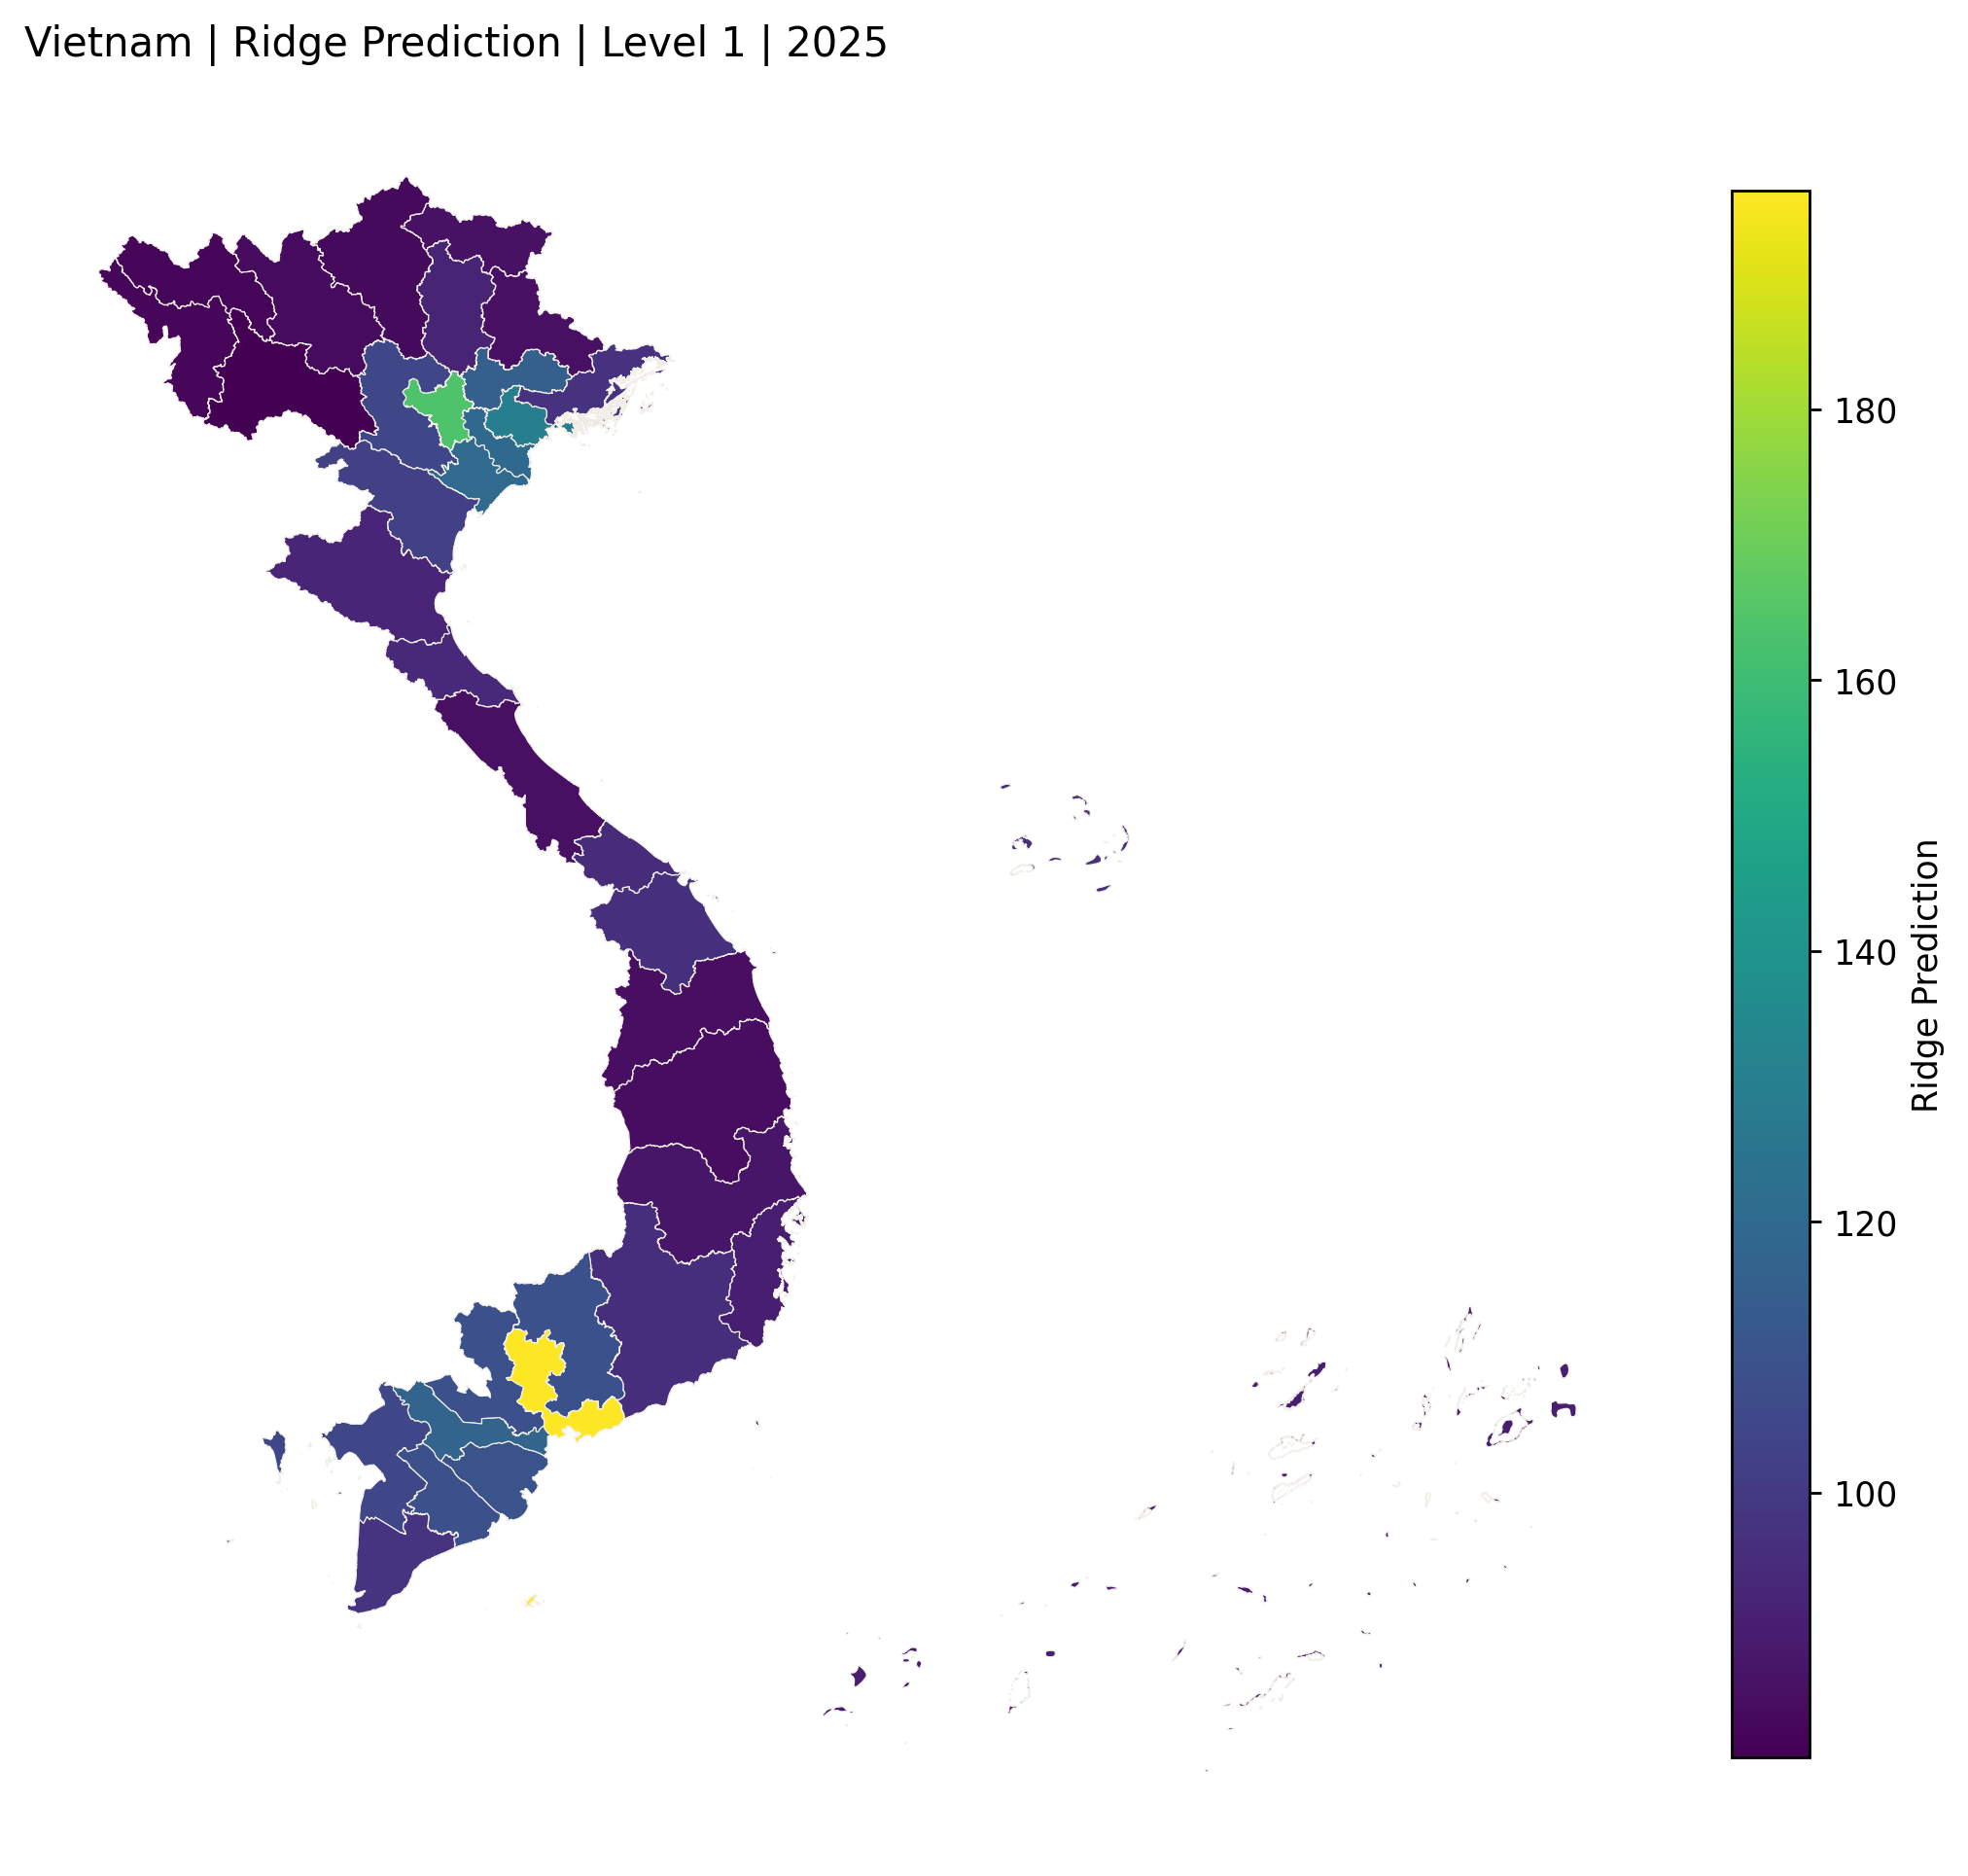
\includegraphics[width=0.5\linewidth]{level1_ridge_2025_holdout_predictions.png}
    \caption{Level 1 predictions: Ho Chi Minh City and Ha Noi have the highest estimated GRDP per capita.}
    \label{fig:level_1_ridge_predictions_2025}
\end{figure}
\begin{figure}
    \centering
    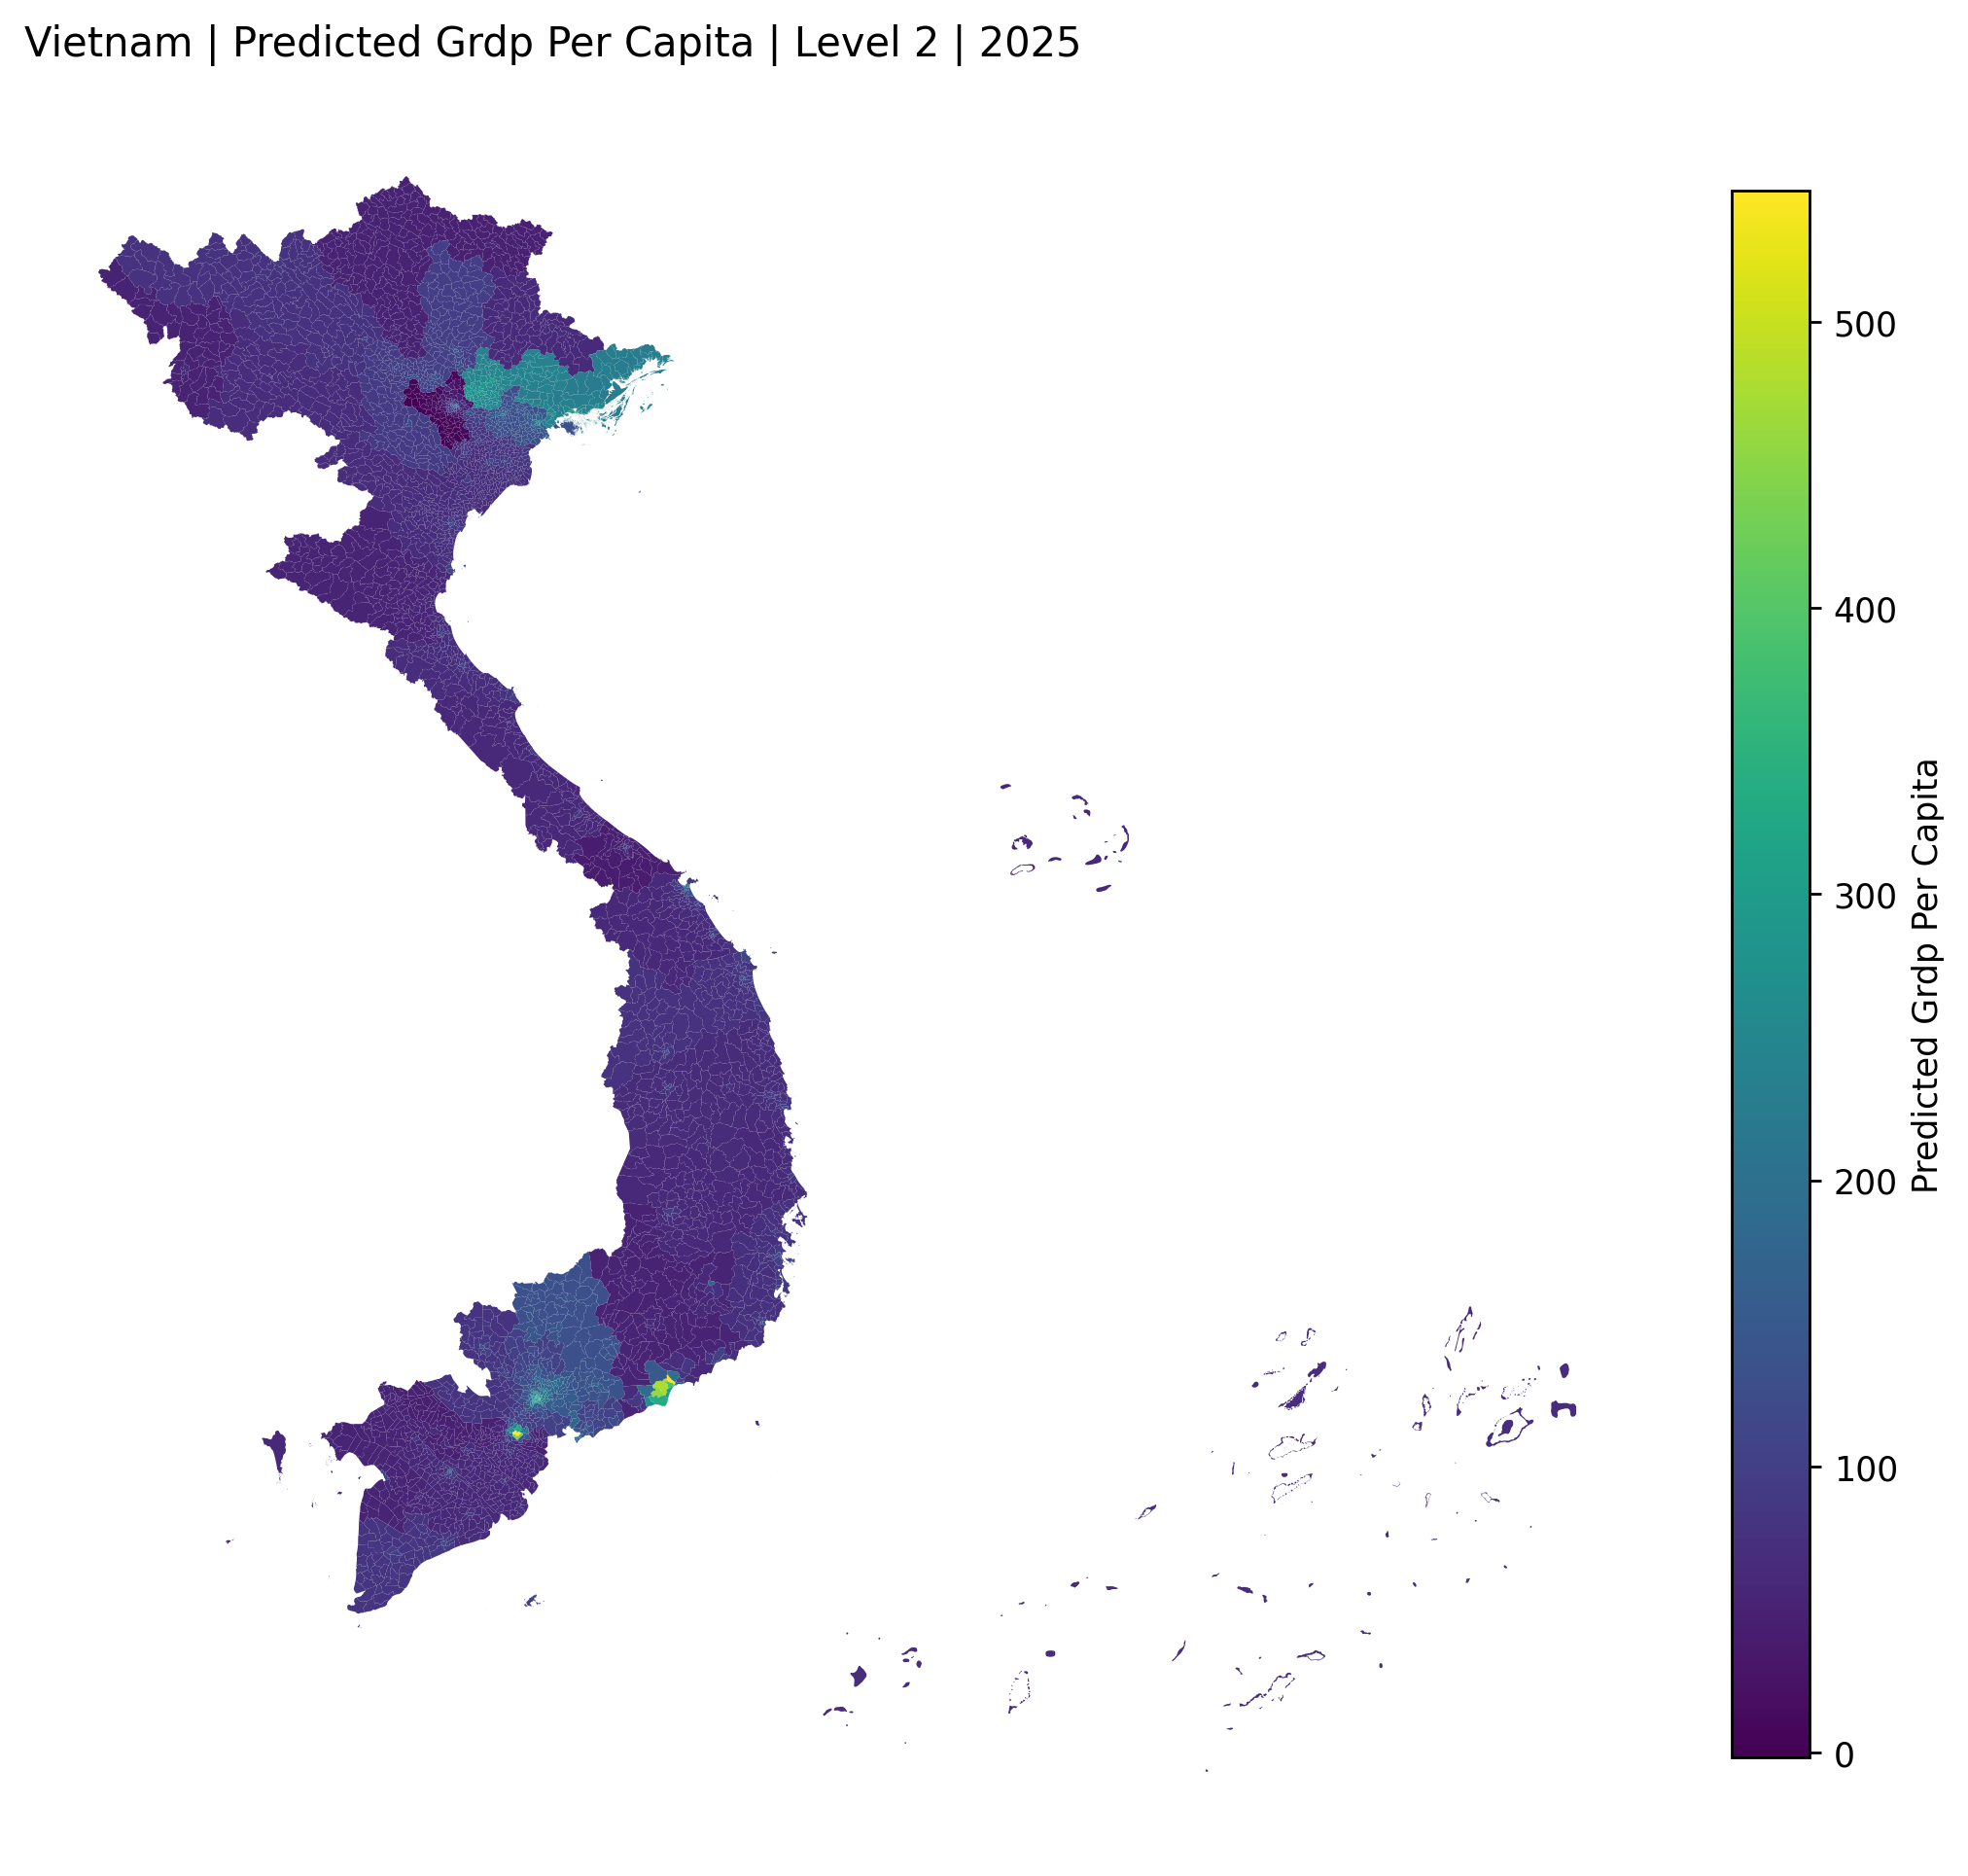
\includegraphics[width=0.5\linewidth]{level2_ridge_2025_holdout_predictions.png}
    \caption{Ridge regression holdout predictions for 2025 at two administrative levels. While Level 1 predictions appear reasonable, Level 2 predictions reveal a potential outlier associated with intensive agricultural lighting in Lam Dong.}
    \label{fig:level_2_ridge_predictions_2025}
\end{figure}


\newpage
% Tells Latex to pull citations from references.bib
\printbibliography % DO NOT CHANGE THIS

\end{document}
